\documentclass[twoside]{article}
\usepackage[T1]{fontenc} 
\usepackage{lmodern}
\input{ISC18-english.sty}
%%%%%%%%%%%%%%%%%%%%%%%%%%%%  Make sure to compile twice for proper cross-references. %%%%%%%%%%%%%%%%%%%%%%%
%%%%%%% For proper display of references, compile the document twice. %%%%%%%%%%%%%%%%%%%%% 
%%%%%%%%%%%%%%% If using TeX Live, compile using pdflatex command %%%%%%%%%%%%%%%%%%%%%%%
\begin{document}
\thispagestyle{empty}
%%%%%%%%%%%%%%%%% Article title header  %%%%%%%%%%%%%%%%%%%%
\fancyhead[LE]{Stress-Strength Reliability for  Discrete Pareto-like Distribution}
%%%%%%%%%%%%%%%%% Article authors header   %%%%%%%%%%%%%%%%%%%%
\fancyhead[RO]{D. Farbod and M. Basirat}
\begin{center}
{
\includegraphics [height=25mm, width=150.3mm] {Images/isc18E}} \\
\vspace*{-1.8cm}
%\begin{center}
%\color{blue} 
%{\hspace{0.1cm}\rule{\textwidth}{1mm}}\\
%\end{center}
\vspace*{4cm}
%%%%%%%%%%%%%%%%% Article title  %%%%%%%%%%%%%%%%%%%%
{\Large \bf  On Stress-Strength Reliability for a Discrete Pareto-like Distribution}\\
 

{\bf
Davood Farbod  \footnote[1]{{\bf Corresponding Author:} {\tt  d.farbod@qiet.ac.ir }}, Maryam Basirat $^2$} \\
$^1$  Department of Mathematics, Faculty of Engineering Science, Quchan University of Technology, Quchan, Iran.\\
$^2$ Department of Mathematics   and Computer Science, Ma.C.,  Islamic Azad Univeristy, Mashhad, Iran.}


\end{center}
\rule{\textwidth}{0.2mm}\\
 
\noindent{\bf Abstract:}\\
In this paper, we  consider   a two-parameter discrete Pareto-like distribution introduced by \cite{Kuznetsov:2001, Kuznetsov:2017}. Basic properties of the model are reviewed, and its asymptotic tail behavior is examined, confirming the Pareto-like heavy-tailed structure. The stress-strength reliability parameter $R=P(X>Y)$ is derived when both stress and strength follow this discrete  distribution. An explicit expression for the reliability measure is obtained in the general case, and a closed-form representation is derived for the identically distributed case. Numerical illustrations are presented to demonstrate the effect of the model parameters on the reliability measure.
 
\noindent{\bf Keywords:} 
discrete Pareto-like distribution,  heavy-tailed distribution, Hurwitz zeta function, stress-strength reliability.\\
\noindent{\bf Mathematics Subject Classification (2010):} $\rm 62E10$, $\rm  60G70$, $\rm 60E05$. \\
\hspace{1cm}\rule{\textwidth}{0.2mm}\\
 
  
\section{Introduction}
Heavy-tailed probability distributions play an important role in modeling complex systems where extreme observations occur with non-negligible probability (see, e.g., \cite{Foss:2013, Kuznetsov:2017}).   Their applications span diverse fields, including bioinformatics, finance, telecommunications, and network science, where empirical data frequently exhibit slow decay in tail behavior. While Pareto and Zeta distributions are classical examples associated with heavy-tailed phenomena, many real-world datasets are inherently discrete. This discrepancy has motivated growing interest in developing and studying discrete counterparts of heavy-tailed models (see, e.g., \cite{Kuznetsov:2017, Kuznetsov:2022}).

The motivation for adopting a discrete framework in the present study is twofold. First, many reliability-related quantities arise naturally in discrete form. In engineering applications, such as failure analysis based on cumulative load cycles or discrete shock occurrences, the variable of interest represents a count rather than a continuous time measure. Modeling such systems using continuous distributions neglects the quantized nature of the state space and may lead to an inaccurate representation of the underlying mechanism. Second, continuous approximations to discrete data may introduce non-negligible distortions in the tail region. Since the present study focuses on distributions with regularly varying tails, accurate characterization of the tail behavior is crucial for reliable statistical inference.

Within reliability theory, an important quantity is the stress–strength parameter $R=P(X>Y)$, where $X$ denotes the strength of a component and $Y$  represents the applied stress, with successful operation defined by $X>Y$. The evaluation of $R$  has been widely studied due to its importance in engineering design and quality control (see, e.g., \cite{Kotz:2003, Kundu:2010}). In recent years, several studies have also investigated stress-strength reliability for discrete distributions (see, e.g., \cite{Bhattacharya:2025a, Bhattacharya:2025b, Choudhury:2021, Imani:2019}). However, compared with the extensive literature on continuous models, stress-strength analysis for discrete distributions remains relatively limited. This is particularly true for discrete heavy-tailed models exhibiting power-law or regularly varying tail behavior. Moreover, in many reliability applications, failure mechanisms are naturally described by event counts (e.g., load cycles or shock occurrences), which further highlights the importance of discrete models for accurately capturing tail behavior.

In this paper, we consider the two-parameter discrete Pareto-like distribution (DPD), originally introduced by \cite{Kuznetsov:2001} and further studied in subsequent works (see also \cite{Astola:2007, Kuznetsov:2017}). This distribution provides a flexible model for discrete data with heavy-tailed and power-law behavior and has been successfully applied in areas such as bioinformatics and complex network analysis. Rather than proposing a new distribution, the aim of the present work is to investigate reliability properties associated with this existing heavy-tailed model. In particular, we derive analytical expressions for the stress-strength reliability when both stress and strength follow the DPD and examine how the tail characteristics of the distribution influence the behavior of the reliability measure. Numerical illustrations are also provided to demonstrate the sensitivity of the stress-strength parameter to the underlying model parameters.


 

 


\subsection{The DPD model} 
We consider the  probability mass function (PMF)  of the two-parameter DPD, where the random variable $X$ follows a $\text{DPD}(\rho, b)$ distribution, as introduced in \cite{Kuznetsov:2001} (see also  \cite{Astola:2007, Kuznetsov:2017}) 
\begin{equation}\label{PMF.DPD} 
p(x;\rho,b) = \frac{(x+b)^{-\rho}}{c(\rho,b)}, \qquad x = 1, 2, \ldots, 
\end{equation} 
where the normalization constant $c(\rho,b)$ is given by 
\begin{equation}\label{normalization} 
c(\rho,b) = \sum_{y=1}^{\infty}(y+b)^{-\rho}. 
\end{equation} 
Here, $\rho > 1$ is the shape parameter and $b > -1$ is the location parameter. The PMF is defined for all positive integers $x$, and the normalization constant ensures that the probabilities sum to one.

\section{Tail Behavior}
The asymptotic tail behavior of a distribution is crucial for assessing the probability of extreme events in stress-strength models, where large observations can significantly influence the reliability parameter $P(X>Y)$.  We therefore examine the tail properties of the DPD model \eqref{PMF.DPD}. Specifically, we prove that the PMF exhibits Pareto-type decay and derive the asymptotic form of the survival function. These results formally confirm the heavy-tailed nature of the DPD distribution.
 

\begin{lem} 
Let $X$ follow a $\mathrm{DPD}(\rho,b)$ distribution with $\rho>1$ and $b>-1$. As $x \to \infty$, the   PMF  \eqref{PMF.DPD} satisfies
\[ 
p(x;\rho,b) \sim \frac{1}{\zeta(\rho,b+1)}\, x^{-\rho},
\] 
where $\sim$   denotes asymptotic equivalence as $x \to \infty$.
\end{lem}

\begin{proof} 
The result follows immediately from the expansion $(x+b)^{-\rho} = x^{-\rho}(1+\frac{b}{x})^{-\rho}$ and the fact that $(1+\frac{b}{x})^{-\rho} \to 1$ as $x \to \infty$.    
\end{proof}

\begin{thm} 
Let $X \sim \mathrm{DPD}(\rho,b)$ with $\rho>1$ and $b>-1$. Then \[ P(X\ge x)\sim \frac{1}{(\rho-1)\,\zeta(\rho,b+1)}\,x^{-(\rho-1)}, \qquad x\to\infty. \] 
\end{thm} 
\begin{proof} 
We have \[ P(X\ge x) = \frac{1}{\zeta(\rho,b+1)} \sum_{k=x}^{\infty} (k+b)^{-\rho} \sim \frac{1}{\zeta(\rho,b+1)} \sum_{k=x}^{\infty} k^{-\rho}. \] 
Using the asymptotic equivalence $\sum_{k=x}^{\infty}k^{-\rho} \sim \frac{x^{-(\rho-1)}}{(\rho-1)}$,  yields the result. 
\end{proof}



\section{Stress-Strength Reliability of the DPD Model} 
Having described the distributional properties and tail behavior of the DPD model, we now study its stress-strength reliability characteristics. Let $X$ and $Y$ be two independent discrete random variables representing the strength and the stress of a system component, respectively. 
Assume that the independent random variables $X$ and $Y$ follow $\mathrm{DPD}(\rho_1, b_1)$ and $\mathrm{DPD}(\rho_2, b_2)$ distributions, respectively.

The stress-strength reliability parameter is defined by $R=P(X>Y)$.   Since $X$ and $Y$ are independent and supported on $\{1,2,3,...\}$, we have \[ R=\sum_{x=1}^{\infty}P(X=x)\,P(Y<x) =\sum_{x=1}^{\infty} p(x;\rho,b)\,F_Y(x-1). \] 
For $\rho>1$, the normalization constant \eqref{normalization} can be expressed in terms of the Hurwitz zeta function as 
\[ 
c(\rho,b)=\zeta(\rho,b+1), 
\] 
where $\zeta(\cdot,\cdot)$ denotes the Hurwitz zeta function. Consequently, the PMF \eqref{PMF.DPD} can be rewritten as (see, e.g., \cite{Kuznetsov:2001})
\[ 
p(x;\rho,b)=\frac{(x+b)^{-\rho}}{\zeta(\rho,b+1)}. 
\]

\begin{thm} 
Let $X$ and $Y$ be independent random variables following $\mathrm{DPD}(\rho_1, b_1)$ and $\mathrm{DPD}(\rho_2, b_2)$ distributions, respectively. The stress-strength reliability is
\begin{equation}\label{S-S-R} 
R = \frac{1}{\zeta(\rho_1, b_1+1)\zeta(\rho_2, b_2+1)} \sum_{x=1}^{\infty} (x+b_1)^{-\rho_1} \sum_{y=1}^{x-1} (y+b_2)^{-\rho_2}. 
\end{equation}
\end{thm} 

\begin{proof} 
By independence, we have  
\begin{equation}\label{1111} 
R = \sum_{x=1}^{\infty} P(X=x) P(Y < x).
\end{equation}
Given $P(X=x) = \frac{(x+b_1)^{-\rho_1}}{\zeta(\rho_1, b_1+1)}$ and $P(Y < x) = \frac{1}{\zeta(\rho_2, b_2+1)} \sum_{y=1}^{x-1} (y+b_2)^{-\rho_2}$, substituting these expressions into  \eqref{1111}  leads directly to \eqref{S-S-R}. This completes the proof. 
\end{proof}


The preceding result provides an exact discrete expression for the reliability parameter without requiring continuous approximations. 

\subsection{Identically distributed case}
We now consider the case where $X$ and $Y$ are independent and identically distributed (i.i.d.) random variables, each with a $\mathrm{DPD}(\rho,b)$ distribution, where $\rho>1$ and $b>-1$.  

\begin{thm}\label{thm:i.i.d} 
If $X$ and $Y$ are i.i.d. $\mathrm{DPD}(\rho,b)$ random variables, the stress-strength reliability is given by  
\begin{equation}\label{R.formula} 
R = \frac{1}{2} \left[ 1 - \frac{\zeta(2\rho, b+1)}{\zeta(\rho, b+1)^2} \right]. 
\end{equation}
\end{thm}
 

\begin{proof} 
Since $X$ and $Y$ are i.i.d., $P(X>Y) = P(Y>X)$. Given $P(X>Y) + P(X<Y) + P(X=Y) = 1$, we have 
\begin{equation}\label{0011} 
R = \frac{1 - P(X=Y)}{2}
\end{equation} 
To evaluate $P(X=Y)$, we compute 
\begin{equation}\label{R.prob.tie} 
P(X=Y) = \sum_{x=1}^{\infty} \left(P(X=x)\right)^2 = \frac{1}{\zeta(\rho, b+1)^2} \sum_{x=1}^{\infty} (x+b)^{-2\rho} = \frac{\zeta(2\rho, b+1)}{\big(\zeta(\rho, b+1)\big)^2}. 
\end{equation}
Substituting  \eqref{R.prob.tie}  into  \eqref{0011}   yields \eqref{R.formula}. 
\end{proof}


 
\begin{cor}\label{cor:RltHalf} 
Under the assumptions of Theorem \ref{thm:i.i.d}, $R < \frac{1}{2}$. This follows from the fact that $P(X=Y) > 0$ for the DPD model \eqref{PMF.DPD}. 
\end{cor}


\subsection{Numerical illustration}
In this subsection, we compute the reliability parameter $R$ for the i.i.d. case using \eqref{R.formula}. The values of the Hurwitz zeta function are computed using the \textsf{R} statistical software \cite{RCore:2026}. Table \ref{tab:R_values} presents $R$ for various values of $\rho$ and $b$. 
 

 

 
\begin{table}[ht] 
\centering 
\caption{Numerical values of $R$ for i.i.d. $\mathrm{DPD}(\rho,b)$ random variables} 
\label{tab:R_values} 
\begin{tabular}{lccccc} \hline & $b=0$ & $b=0.5$ & $b=1$ & $b=2$ & $b=5$ \\ \hline $\rho=1.5$ & 0.4106 & 0.4443 & 0.4602 & 0.4749 & 0.4882 \\ $\rho=2$ & 0.3000 & 0.3656 & 0.4010 & 0.4364 & 0.4700 \\ $\rho=2.5$ & 0.2119 & 0.2923 & 0.3417 & 0.3954 & 0.4497 \\ $\rho=3$ & 0.1480 & 0.2303 & 0.2876 & 0.3553 & 0.4290 \\ $\rho=4$ & 0.0714 & 0.1399 & 0.1992 & 0.2823 & 0.3879 \\ \hline 
\end{tabular} 
\end{table}


\begin{prop} 
For i.i.d. random variables $X$ and $Y$ following a $\mathrm{DPD}(\rho, b)$ distribution, the reliability $R$ is an increasing function of $b$ and a decreasing function of $\rho$. 
\end{prop} 

As shown in Table \ref{tab:R_values}, for a fixed $\rho$, $R$ increases with $b$ and approaches $0.5$. Conversely, for a fixed $b$, $R$ decreases as $\rho$ increases. This behavior is consistent with \eqref{R.formula}:  higher values of $\rho$ shift the probability mass toward smaller integers, thereby increasing the probability $P(X=Y)$  and consequently reducing $R$.   The variation of $R$ with respect to $b$ for different values of $\rho$ is illustrated in Figure \ref{fig:R_plot}. 
 


\begin{center}
 
\begin{figure}[h]
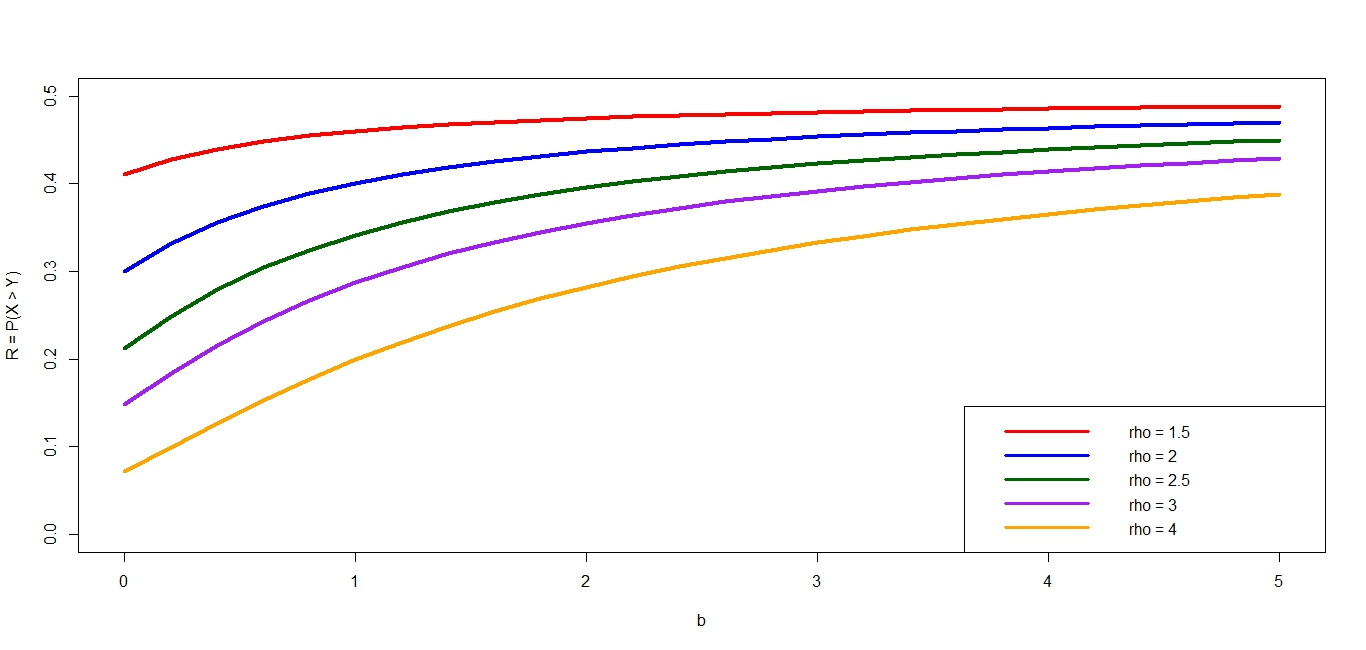
\includegraphics[width=0.9\textwidth]{Figure1.jpeg}\\ 
\caption{The reliability $R = P(X>Y)$ as a function of $b$ for various values of $\rho$.}
\label{fig:R_plot}
\end{figure}
 
\end{center} 


\section{Conclusion}
In this paper, we investigated the stress-strength reliability of the two-parameter discrete Pareto-like distribution (DPD) model \eqref{PMF.DPD}. The asymptotic analysis showed that both the PMF and the survival function exhibit Pareto-type decay, confirming the heavy-tailed character of the distribution.

An explicit expression for the reliability parameter $R=P(X>Y)$  was derived in the general case, while in the identically distributed setting a closed-form representation in terms of the Hurwitz zeta function was obtained. It was also shown that $R<0.5$  in the i.i.d. case. Numerical investigations further illustrated the effects of the parameters  $\rho$ and $b$ on the reliability measure.

Since much of the existing stress-strength reliability literature has focused on continuous models, the present study emphasized the relevance of discrete heavy-tailed distributions in reliability analysis. The results showed that the DPD model \eqref{PMF.DPD} provides a useful framework for reliability problems involving discrete data with power-law tail behavior, and thus contributes to the still limited literature on stress-strength reliability for discrete heavy-tailed models.

Several directions remain open for future research, including the development of statistical inference procedures for the reliability parameter, extensions to dependent stress-strength models, and the study of other discrete heavy-tailed distributions within the same reliability framework.


\begin{thebibliography}{99}
\bibitem[Astola and Danielian (2007)]{Astola:2007}
Astola, J.  and  Danielian, D.  (2007),  {\it Frequency distributions in biomolecular systems and growing networks}, Tampere International Center for Signal Processing (TICSP),  Series no. 31.  Tampere, Finland. 

\bibitem[Bhattacharya and  Bhattacharjee (2025a)]{Bhattacharya:2025a}
Bhattacharya, R. and Bhattacharjee, M. (2025a),  A  modified  stress-strength  reliability  function  for discrete  family of  distributions,
 \textit{International Journal of Reliability, Quality and  Safety Engineering},  \textbf{32}(3), p. 1. 

\bibitem[Bhattacharya and  Bhattacharjee (2025b)]{Bhattacharya:2025b}
Bhattacharya, R. and  Bhattacharjee, M. (2025b),  Stress-strength reliability for discrete distributions: an alternative formulation, \textit{Life Cycle Reliability and Safety Engineering}, \textbf{14}(2), 205-214.

\bibitem[Choudhury et al. (2021)]{Choudhury:2021}
Choudhury, M. M., Bhattacharya, R. and  Maiti, S. S.  (2021), On estimating reliability function for the family of power series distribution, \textit{Communications in Statistics-Theory and Methods}, \textbf{50}(12), 2801-2830.
  
\bibitem[Danielian and Astola (2007)]{Danielian:2007}
Danielian, E. and Astola, J. (2007), On generating functions of Pareto and Waring distributions, In: R. Bregovic and A. Gotchev (eds.),  \textit{Proceedings 2007  International TICSP Workshop on Spectral Methods and Multirate Signal Processing}, Moscow, Russia, 1-2 September,  235-237.
 
\bibitem[Farbod (2015)]{Farbod:2015}
Farbod, D. (2015), On the estimators for some frequency distributions arising in bioinformatics, \textit{Bulletin of the Georgian National Academy of Sciences}, \textbf{9}(1), 44-50.

\bibitem[Foss (2013)]{Foss:2013}
Foss, S., Korshunov, D.  and  Zachary, S. (2013),  \textit{An Introduction to Heavy-Tailed and Subexponential Distributions}, Springer.

\bibitem[Imani and  Khorashadizade (2019)]{Imani:2019}
Imani, M. and  Khorashadizadeh, M.  (2019),  On estimation of stress-strength parameter for discrete Weibull distribution, \textit{In Paper presented at  the   5-th Seminar on Reliability Theory and its Applications}, pp. 142, Yazd University, Iran.


\bibitem[Kotz et al. (2003)]{Kotz:2003}
Kotz, S., Lumelskii, Y. and Pensky, M. (2003), \textit{The Stress-Strength Model and Its Generalizations: Theory and Applications}, World Scientific, Singapore.

\bibitem[Kundu and Gupta (2010)]{Kundu:2010} 
Kundu, D. and Gupta, R. D. (2010), Estimation of $P(Y<X)$ for generalized exponential distribution, \textit{Metrika}, \textbf{72}, 169-191.

\bibitem[Kuznetsov (2001)]{Kuznetsov:2001}
Kuznetsov, V. A. (2001), Distribution associated with stochastic processes of gene expression in a single eukaryotic cell,  \textit{EURASIP Journal on Applied Signal Processing},   \textbf{4}, 285-296.

\bibitem[Kuznetsov (2017)]{Kuznetsov:2017}
Kuznetsov, V. A. (2017), {\it Mathematical modeling of avidity distribution and estimating general binding properties of transcription factors from genome-wide binding profiles}, In: Tatarinova,T. V. and Nikolsky, Y. (eds), Biological Networks and Pathway Analysis, pp. 193-276, Springer, New York.

\bibitem[Kuznetsov et al. (2022)]{Kuznetsov:2022}
Kuznetsov, V. A., Grageda, A. and  Farbod, D. (2022), Generalized hypergeometric distributions generated by birth-death process in bioinformatics, {\it Markov Processes and Related Fields}, \textbf{28}(2), 303-327.

\bibitem[RCore (2026)]{RCore:2026}
R Core Team.   (2026),  \textit{R: A Language and Environment for Statistical Computing},  R Foundation for Statistical Computing.

\end{thebibliography}

 \end{document}

